\section{Modules}

To implement a soft RISC-V processor, I created several modules that work together to form the complete system.
Each module is responsible for a specific part of the processor's functionality.
In this section, I will describe each module briefly, including its purpose and how it interacts with other modules.

\subsection{Types}

The `types.sv` file contains various enumerations and constants used throughout the design.
These include the instruction types, CPU states, RV32I op codes, funct3 bits, funct7 bits, and ALU control signals.
Although SystemVerilog supports a convenient way to export this module as a package, since `yosys` does not support this feature, I had to use a workaround by converting every `.sv` file to a `v` file using
\href{https://github.com/zachjs/sv2v}{`sv2v`}.


\subsection{Arithmetic Logic Unit (ALU)}

\begin{figure}[H]
    \centering
    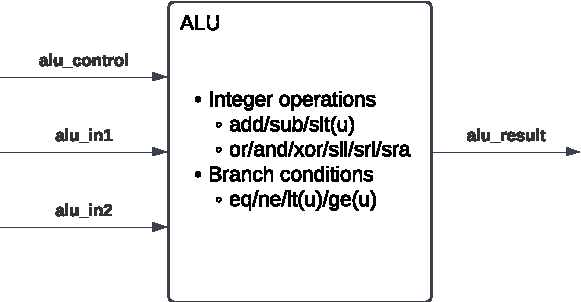
\includegraphics[width=0.6\textwidth]{media/alu}
    \caption{ALU}
    \label{fig:alu}
\end{figure}

The ALU performs arithmetic and logical operations such as addition, subtraction, bitwise operations, and comparisons for R-type, I-type, and B-type instructions.
It takes two operands and a control signal to determine which operation to execute.

\subsection{Control Unit}

\begin{figure}[H]
    \centering
    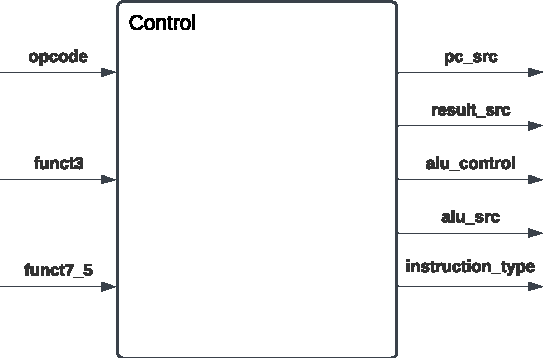
\includegraphics[width=0.6\textwidth]{media/control}
    \caption{Control unit}
    \label{fig:control}
\end{figure}

The control unit decodes the instruction opcode and generates all necessary control signals for various multiplexers in the system -- ALU operation, program counter updates, and register file write data source.

\subsection{Immediate Extender}

\begin{figure}[H]
    \centering
    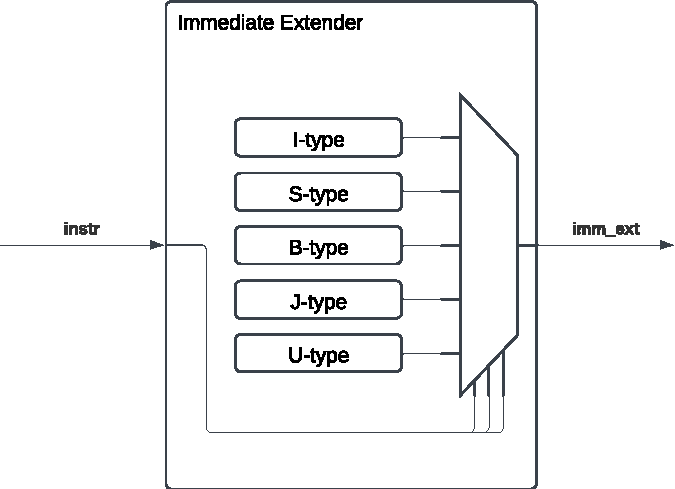
\includegraphics[width=0.6\textwidth]{media/imm_extender}
    \caption{Immediate extender}
    \label{fig:immgen}
\end{figure}

The immediate extender takes the instruction and generates the immediate value based on opcode (the instruction type).
The extended immediate value is used for address calculations, branch offsets, and immediate values for ALU operations, etc.

\subsection{Register File}

\begin{figure}[H]
    \centering
    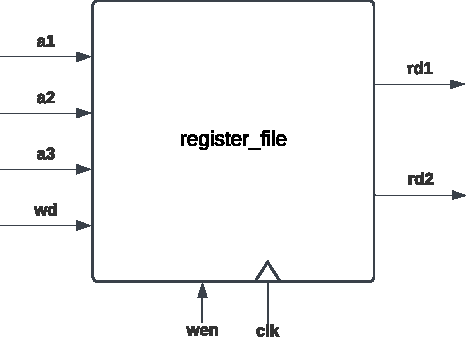
\includegraphics[width=0.6\textwidth]{media/register_file}
    \caption{Register file}
    \label{fig:regfile}
\end{figure}

The register file contains 32 registers, where the 0th register is hardcoded to zero.
It supports two simultaneous reads and one write operation.
Although reads occur combinationally, writes occur synchronously at the rising edge of the clock.

\subsection{Program Counter Selector}

\begin{figure}[H]
    \centering
    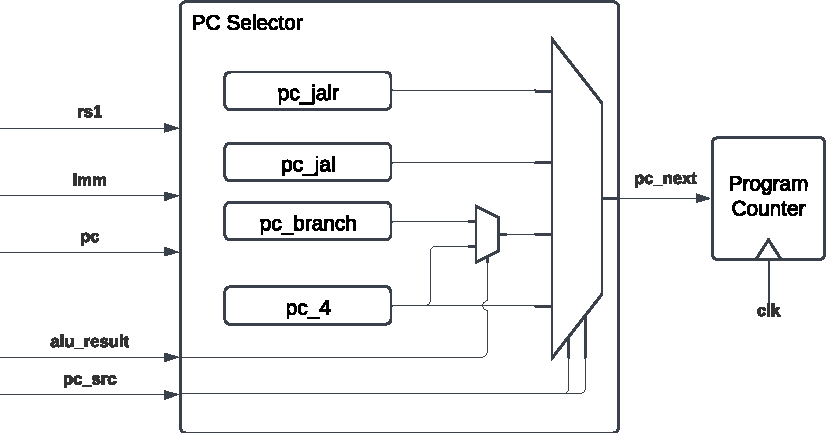
\includegraphics[width=0.8\textwidth]{media/pc_selector}
    \caption{Program counter selector}
    \label{fig:pcselector}
\end{figure}

The program counter selector computes the all four possible next addresses, and outputs the selected one based on the control signal.
The four possible cases are:
\begin{itemize}
    \item rs1 + immediate (JALR)
    \item PC + immediate (JAL)
    \item PC + immediate (branch when taken)
    \item PC + 4 (default case)
\end{itemize}